% !TeX TXS-program:compile = txs:///pdflatex/[--shell-escape]
\pdfoptionpdfminorversion=5
\documentclass[10pt, aspectratio=169, t ,hyperref={pdfpagelabels=false}]{beamer}
\usepackage{pgfpages}
%\setbeameroption{show notes on second screen=right}

\mode<presentation> {
    \usetheme{HHUD}
    \setbeamercovered{invisible}
}
\usepackage[ngerman]{babel}
\usepackage[utf8]{inputenc}
\usepackage{times}
\usepackage[T1]{fontenc}
\usepackage{amsmath}
\usepackage{subfigure}
\usepackage{graphicx}
\usepackage{hyperref}
\usepackage{xmpmulti}
\usepackage{multicol}
\usepackage{icomma}
\usepackage{csquotes}
\usepackage{listings}
\usepackage{minted}
\usepackage[backend=bibtex,style=verbose,url=false]{biblatex}
\bibliography{lit}
% If you want to exclude the appendix from the frame counter you have to use the appendixnumberbeamer package. But be aware that the current version causes a problem with the frame counter.
\usepackage{appendixnumberbeamer}

%% Die folgenden Zeilen können auskommentiert werden, um vor jedem Kapitel eine Gliederungsfolie einzufügen
% \AtBeginSection[] {
%   \begin{frame}<beamer>
%     \thispagestyle{empty}
%     \frametitle{Gliederung}
%     \vspace{-5mm}
%     \tableofcontents[currentsection]
%   \end{frame}
% }

\usebackgroundtemplate{\includegraphics[width=\paperwidth]{fig/background_cd_2020}}

\newcommand{\backgroundNormal}{\usebackgroundtemplate{
    \includegraphics[width=\paperwidth]{fig/background_cd_2020}}}
\newcommand{\backgroundTitle}{\usebackgroundtemplate{
    
\includegraphics[width=\paperwidth]{fig/background_heine}}}
\newcommand{\backgroundEmpty}{\usebackgroundtemplate{
    
\includegraphics[width=\paperwidth]{fig/background_empty}}}
    
\setlength{\leftmargini}{9pt}
\setbeamersize{text margin left=25pt,text margin right=25pt} 
\setbeamertemplate{itemize/enumerate subbody end}{\vspace{.5\baselineskip}}

% % % % % % % % % %  CHANGE TOPIC AND AUTHOR INFORMATION HERE % % % % % % % % %
\newcommand{\abschluss}{Bachelor}                              % HIER UNZUTREFFENDES LÖSCHEN
\title{\abschluss{}arbeit:\\Diffusionsmodelle zur Vorhersage der tertiären Struktur von RNA
}                      % HIER DEN TITEL DER ARBEIT EINTRAGEN
\author{Sven Klein}                                                       % HIER DEN NAMEN UND VORNAMEN EINTRAGEN
\date{DATUM}                                                                % HIER DAS PRÄSENTATIONSDATUM EINTRAGEN
% % % % % % % % % % % % % % % % % % % % % % % % % % % % % % % % % % % % % % % %
\institute{Mathematische Modellierung Biologischer Systeme\\Heinrich-Heine-Universität Düsseldorf}
\subject{Informatik}

%
% Hier beginnt das Dokument
%
\begin{document}

\backgroundTitle
  \begin{frame}
    \thispagestyle{empty}
    \begin{columns}
    \column{0.4\paperwidth}
    {
    \footnotesize
    \color{hhuBlau}
    \put(20,-200){\insertdate}
    
    }
    \column{0.6\paperwidth}
    
    \color{hhuBlau}
    \LARGE \inserttitle\\[\baselineskip]
    
    \large \insertauthor
    \end{columns}
  \end{frame}
  \backgroundNormal

  % % % % % % % % % % Ab hier werden die LaTeX-Dateien der einzelnen Abschnitte eingefügt % % % % % % % % % %

  \section{RNA Basics}
\begin{frame}{Was ist RNA?}
	\begin{itemize}
			\item RNA besteht aus einer Aneinandereihung von Nukleotiden
			\item Die Nukleotide bestehen aus einer Base, Ribose und einem Phosphat.
			\item Es gibt vier verschiedene mögliche Basen Adenin (A), Guanin (G), Cytosin (C) und Uracil (U)
			\item Die Kombination aus Ribose und Phosphat wird auch als Backbone bezeichnet
			\item RNA ist zum Beispiel bei der Herstellungen von Proteinen beiteiligt und liefert dabei genetische Informationen in Form von mRNA.
	\end{itemize}
\end{frame}

\begin{frame}{RNA - Primärstruktur}
\vspace*{\fill}
\begin{figure}
	\includegraphics[width=1\textwidth]{imgs/pst.png}
\end{figure}	
\vspace*{\fill}
\end{frame}

\begin{frame}{RNA - Sekundärstruktur}
\vspace*{\fill}
\begin{figure}
	\includegraphics[width=0.7\textwidth]{imgs/sst.png}
\end{figure}	
\vspace*{\fill}
\end{frame}

\begin{frame}{RNA - Tertiärstruktur}
\vspace*{\fill}
\begin{figure}
	\includegraphics[width=.4\textwidth]{imgs/tst.png}
\end{figure}	
\vspace*{\fill}
\end{frame}

\begin{frame}{Warum braucht man die Tertiärstruktur?}
	Über die Tertiärstruktur erfährt man vieles über die Eigenschaften der RNA wie zum Beispiel
	\begin{itemize}
			\item Funktion
			\item Ineraktion mit anderen Molekülen
			\item Stabilität
	\end{itemize}
	\vspace{.5cm}
	Die Tertiärstruktur hat einige praktische Anwendungen:
	\begin{itemize}
			\item Biologische Prozesse verstehen
			\item Design eigener RNA die gewünschte Funktion hat (z. B. RNA-Impfstoff)
	\end{itemize}

\end{frame}


  \section{Diffusion}
\begin{frame}{Warum Diffusionsmodelle?}
	\begin{itemize}
	\item Diffusionsmodelle sind generative Modelle, welche in der Regel dazu genutzt werden Bilder zu generieren.
	\item Es können beliebig viele verschiedene Ausgaben generiert werden
	\item RNA kann bei gleicher Primärstruktur mehrere verschiedene Tertiärstrukturen haben
	\item Diffusionsmodelle liefern in der Regel sehr gute Ergebnisse im Vergleich zu anderen generativen Modellen
	\end{itemize}
\end{frame}

\begin{frame}{Wie funktionieren Diffusionsmodelle? - Überblick}
	\begin{itemize}
		\item Bilder $\boldsymbol y$ folgen einer Verteilung $p_{\text{data}}(\boldsymbol y)$
		\item Ziel ist es den Gradienten $\boldsymbol \nabla_{\boldsymbol x} \, p_\text{data}(\boldsymbol x)$ zu lernen.
		\item Generiere neue Bilder indem man mit zufälligen Pixelwerten startet und diese dann in Richtung des Gradienten $\boldsymbol \nabla_{\boldsymbol x} \, p_\text{data}(\boldsymbol x)$ verändert.
	\end{itemize}
\end{frame}

\begin{frame}{Wie funktionieren Diffusionsmodelle? - Überblick}
\vspace*{\fill}
\begin{figure}
        \includegraphics[width=.35\textwidth]{imgs/samplingpath.png}
\end{figure}    
\vspace*{\fill}
\end{frame}
\begin{frame}{Wie funktionieren Diffusionsmodelle? - Training}
	\begin{enumerate}
		\item Wähle ein Bild $\boldsymbol y$ aus den Trainingsdaten.	
		\item Generiere verrauschtes Bild $\hat{\boldsymbol y}$, indem man ein zufälliges Rauschen $\boldsymbol n \sim \mathcal{N}(\boldsymbol 0, \sigma \boldsymbol I)$ aufaddiert, wobei $\sigma$ zufällig aus der Verteilung $\sigma_{\text{train}}$ gewählt wird.
		\item Benutze das Netzwerk $\boldsymbol D$ um aus dem verrauschten Bild $\hat{\boldsymbol y}$ eine Vorhersage $\boldsymbol x$ des ursprünglichen Bildes zu erhalten.
		\item Optimiere Netzwerkparameter basierend auf dem Fehler $\lambda(\sigma) \lVert \boldsymbol D(\boldsymbol y + n, \sigma) - \boldsymbol y \rVert^2_2$
	\end{enumerate}
\end{frame}

\begin{frame}{Wie funktionieren Diffusionsmodelle? - Training}
\vspace*{\fill}
\begin{figure}
        \includegraphics[width=.8\textwidth]{imgs/sigma_loss.png}
\end{figure}    
\vspace*{\fill}
\end{frame}

\begin{frame}{Wie funktionieren Diffusionsmodelle? - Sampling}
	\begin{enumerate}
		\item Wähle $0 = \sigma_0 < \sigma_1 < ... < \sigma_n$
		\item Starte mit Rauschen $\boldsymbol x_n \sim \mathcal{N}(\boldsymbol 0, \sigma_n \boldsymbol I)$ 
		\item Generiere $\boldsymbol x_{n-1} = \boldsymbol x_n + \frac{\sigma_n - \sigma_{n-1}}{\sigma_n} \left (\boldsymbol x_n - \boldsymbol D(\boldsymbol x_n, \sigma_n) \right )$
		\item Fertiges Bild ist $\boldsymbol x_0$
	\end{enumerate}
\end{frame}
\begin{frame}{Wie funktionieren Diffusionsmodelle? - Sampling}
\vspace*{\fill}
\begin{figure}
	\includegraphics[width=.7\textwidth, trim={0 1cm 0 1.5cm}, clip]{imgs/denoising.png}
\end{figure}    
\vspace*{\fill}
\end{frame}
\begin{frame}{Wie funktionieren Diffusionsmodelle? - Ergebnisse}
\vspace*{\fill}
\begin{figure}
	\includegraphics[width=.35\textwidth, trim={0 3cm 0 1.5cm}, clip]{imgs/generated_images.png}
\end{figure}    
\vspace*{\fill}
\end{frame}


  \begin{frame}{Datenvorbereitung}
Daten kommen aus dem Paper "De novo prediction of RNA 3D structures with deep generative models" von J. Ramakers,  F. Blum, S. König, S. Harmeling und M. Kollmann
\begin{enumerate}
\item Lade alle RNA Strukturen aus der RNASolo Datenbank herunter
\item Entferne alle Strukturen, die Bindungen zu DNA, einem Protein oder einer anderen RNA haben.
\item Spalte große komplizierte RNA Strukturen in einzelne Stränge auf
\item Bilde Cluster  mit maximaler Sequenzidentität von 70\%
\item Teile Daten basierend auf den Clustern in Trainings-, Validierungs- und Testdaten auf.
\item Schneide zufällige Teile der RNA raus, sodass die Gesamtlänge maximal 96 Nukleotide beträgt. Behalte nur Ausschnitte bei denen die Anzahl der Nukleotide, die eine Bindung zu einem abgeschnitten Teil der RNA haben, maximal 5\% beträgt.
\end{enumerate}
\end{frame}

\begin{frame}{Datenrepräsentation}
\begin{itemize}
\item Für jedes Nukleotide werden die Koordinaten von 3 Atomen in der Base und 2 Atomen im Backbone betrachtet
\item Da die Koordinaten weder translations- noch rotationsinvariant sind wird daraus nun eine Distanzmatrix berechnet.
\item Die Distanzmatrizen werden nun vom Diffusionsmodell gelernt
\item Die vom Diffusionsmodell generierten Distanzmatrizen werden mithilfe von MDS wieder in Koordinaten umgewandelt.
\end{itemize}
\end{frame}

  \appendix

  \section{Anhang}

\subsection{Subsection kann auch leer gelassen werden.}

\begin{frame}
  \frametitle{Sinn des Anhangs}

  In Diskussionen nach Präsentationen kommt es häufiger vor, dass Nachfragen
  gestellt werden, die mit dem regulären Material der Präsentation nicht zu
  beantworten sind.

  Daher lohnt es sich, zusätzliche
  \begin{itemize}
    \item Grafiken
    \item Tabellen mit Detailinformationen
    \item Erklärungen
  \end{itemize}
  aus der schriftlichen Arbeit im Anhang unterzubringen.

\end{frame}


  % % % % % % % % % % Ende der eingefügten LaTeX-Dateien % % % % % % % % % %

\end{document}

%
% Hier endet das Dokument
%
